\documentclass[11pt]{article}
\usepackage[a4paper,margin=0.9in]{geometry}
\usepackage{amsmath,amssymb,amsthm,mathtools}
\usepackage{graphicx}
\usepackage[hidelinks]{hyperref}
\usepackage{microtype}

\newtheorem{theorem}{Theorem}
\newtheorem{lemma}{Lemma}
\newcommand{\PW}{\operatorname{PW}}
\newcommand{\cL}{\mathcal L}
\newcommand{\one}{\mathbf 1}

\title{A uniqueness set which is not sampling and whose\\
complement is not a \(\lambda\)-set}
\author{Candidate full counterexample packet for arXiv:2511.17343}
\date{17 August 2026}

\begin{document}
\maketitle

\begin{abstract}
Under exactly the graph assumptions stated by Giannoni, there is a positive
bandwidth \(\omega\), an infinite-dimensional Paley--Wiener space
\(\PW_\omega(G)\), and a uniqueness set \(W\) whose complement is not a
\(\lambda\)-set.  In fact, \(W\) is not a sampling set and
\((\PW_\omega(G),\|\cdot\|_W)\) is incomplete.  The graph is the disjoint
union of an eight-cycle and finite 10-regular Ramanujan expanders of unbounded
order.  The proof reduces to exact finite-graph spectral calculations and one
explicit family of test functions.
\end{abstract}

\paragraph{Status and scope.}
This is a candidate full affirmative answer to the existence question following
source Theorem~3.1, together with a negative answer to the completeness issue
raised after source Theorem~2.8.  The source assumes countably many vertices,
no isolated vertices, simple undirected uniformly weighted edges, and finite
maximum degree; it does not assume that the graph is connected.  The example
uses this stated generality.  A connected version is not claimed.

\section{Construction and spectral calculation}

For a regular graph of degree \(d\), the normalized Laplacian used in the
source is
\[
  \cL=I-\frac1d A,
\]
where \(A\) is the adjacency operator.  Let \((X_n)_{n\ge1}\) be connected
10-regular bipartite Ramanujan graphs of orders \(N_n\) tending to infinity.
Passing to a subsequence, assume \(N_n\ge n^4\).  Such an infinite family
exists by Marcus--Spielman--Srivastava~\cite{MSS}.  Put
\[
  G=C_8\;\sqcup\;\bigsqcup_{n\ge1}X_n,
  \qquad \omega=1-\frac1{\sqrt2}>0.
\]
This is a simple, uniformly weighted, countable graph without isolated
vertices and with maximum degree 10.

The adjacency eigenvalues of \(C_8\) are
\(2\cos(2\pi k/8)\), \(0\le k<8\).  Hence the normalized-Laplacian
eigenvalues are
\[
  1-\cos(2\pi k/8),
\]
so \(\omega\) is an eigenvalue of multiplicity two and
\(\dim\PW_\omega(C_8)=3\).  In particular \(\omega\in\sigma(\cL_G)\), as
required in the source definition of uniqueness set.

On every \(X_n\), the constant functions form the zero eigenspace.  Every
nontrivial adjacency eigenvalue \(\mu\) satisfies
\(|\mu|\le2\sqrt{10-1}=6\); therefore every nonzero normalized-Laplacian
eigenvalue is at least
\[
  1-\frac6{10}=\frac25
  \;>\;1-\frac1{\sqrt2}=\omega.
\]
The spectral projection of a Hilbert direct sum is the direct sum of the
component spectral projections.  Consequently
\begin{equation}\label{eq:PW}
 \PW_\omega(G)
 =\PW_\omega(C_8)\oplus
   \bigoplus_{n\ge1}\operatorname{span}\{\one_{X_n}\}.
\end{equation}
Thus this Paley--Wiener space is infinite-dimensional.  Every one of its
elements has a unique representation
\begin{equation}\label{eq:representation}
 f=g\oplus\bigoplus_{n\ge1}c_n\one_{X_n},\qquad
 g\in\PW_\omega(C_8),\qquad
 \|g\|_2^2+\sum_{n\ge1}N_n|c_n|^2<\infty.
\end{equation}

\section{The full counterexample}

Choose one vertex \(x_n\in X_n\) for each \(n\), and define
\[
  W=V(C_8)\cup\{x_n:n\ge1\},\qquad S=V(G)\setminus W.
\]

\begin{theorem}\label{thm:main}
For \(G,\omega,W,S\) above:
\begin{enumerate}
 \item \(W\) is a uniqueness set for \(\PW_\omega(G)\);
 \item \(W\) is not a sampling set;
 \item \((\PW_\omega(G),\|\cdot\|_W)\) is not complete;
 \item \(S\) is not a \(\lambda\)-set for any finite \(\lambda\).
\end{enumerate}
\end{theorem}

\begin{proof}
For \(f\) as in \eqref{eq:representation}, restriction to \(W\) gives all
values of \(g\) and the single value \(c_n=f(x_n)\) on each \(X_n\).  Hence
\(f|_W=0\) implies \(g=0\) and every \(c_n=0\), proving uniqueness.  Moreover,
the two norms have the exact forms
\begin{align}
 \|f\|_2^2&=\|g\|_2^2+\sum_{n\ge1}N_n|c_n|^2,\label{eq:ambient}\\
 \|f\|_W^2&=\|g\|_2^2+\sum_{n\ge1}|c_n|^2.\label{eq:sampling}
\end{align}

Let \(h_n=N_n^{-1/2}\one_{X_n}\), extended by zero off \(X_n\).  Then
\(h_n\in\PW_\omega(G)\), \(\|h_n\|_2=1\), and
\(\|h_n\|_W=N_n^{-1/2}\to0\).  No uniform lower frame inequality is
possible, so \(W\) is not sampling.

For incompleteness, let
\[
 f^{(m)}=\bigoplus_{n=1}^{m}\frac1n\one_{X_n}.
\]
Every \(f^{(m)}\) lies in \(\PW_\omega(G)\), and \eqref{eq:sampling} shows
that \((f^{(m)})\) is Cauchy in \(\|\cdot\|_W\).  If it converged in that
norm to some \(f\in\PW_\omega(G)\), then coordinate convergence at \(x_n\)
would force the coefficient of \(\one_{X_n}\) in \(f\) to be \(1/n\) for
every \(n\).  But then \eqref{eq:ambient} and \(N_n\ge n^4\) give
\[
 \|f\|_2^2\ge\sum_{n\ge1}\frac{N_n}{n^2}
 \ge\sum_{n\ge1}n^2=\infty,
\]
a contradiction.

It remains to test the \(\lambda\)-set inequality directly.  Let \(\varphi_n\)
be one on \(X_n\setminus\{x_n\}\) and zero everywhere else.  It is supported
in \(S\) and
\[
 \|\varphi_n\|_2^2=N_n-1.
\]
Because \(X_n\) is 10-regular, \(\cL\varphi_n\) equals \(-1\) at \(x_n\),
equals \(1/10\) at each of its ten neighbors, and is zero at every other
vertex.  Therefore
\[
 \|\cL\varphi_n\|_2^2=1+10\left(\frac1{10}\right)^2=\frac{11}{10}.
\]
The ratio \(\|\varphi_n\|_2/\|\cL\varphi_n\|_2\) tends to infinity, so no
finite Poincar\'e constant \(\lambda\) works on \(S\).
\end{proof}

\paragraph{What the example resolves.}
The paper asks whether uniqueness sets not arising as complements of
\(\lambda\)-sets exist.  Theorem~\ref{thm:main} supplies one at a genuine
positive spectral bandwidth.  It simultaneously shows why uniqueness alone
does not imply stable sampling: injectivity of the restriction map does not
make its range closed.  Equations \eqref{eq:ambient}--\eqref{eq:sampling}
identify the defect exactly as the missing component-size weights.

\section{Source evidence}

The source first identifies completeness of the uniqueness norm as unknown
(PDF page 8):
\begin{center}
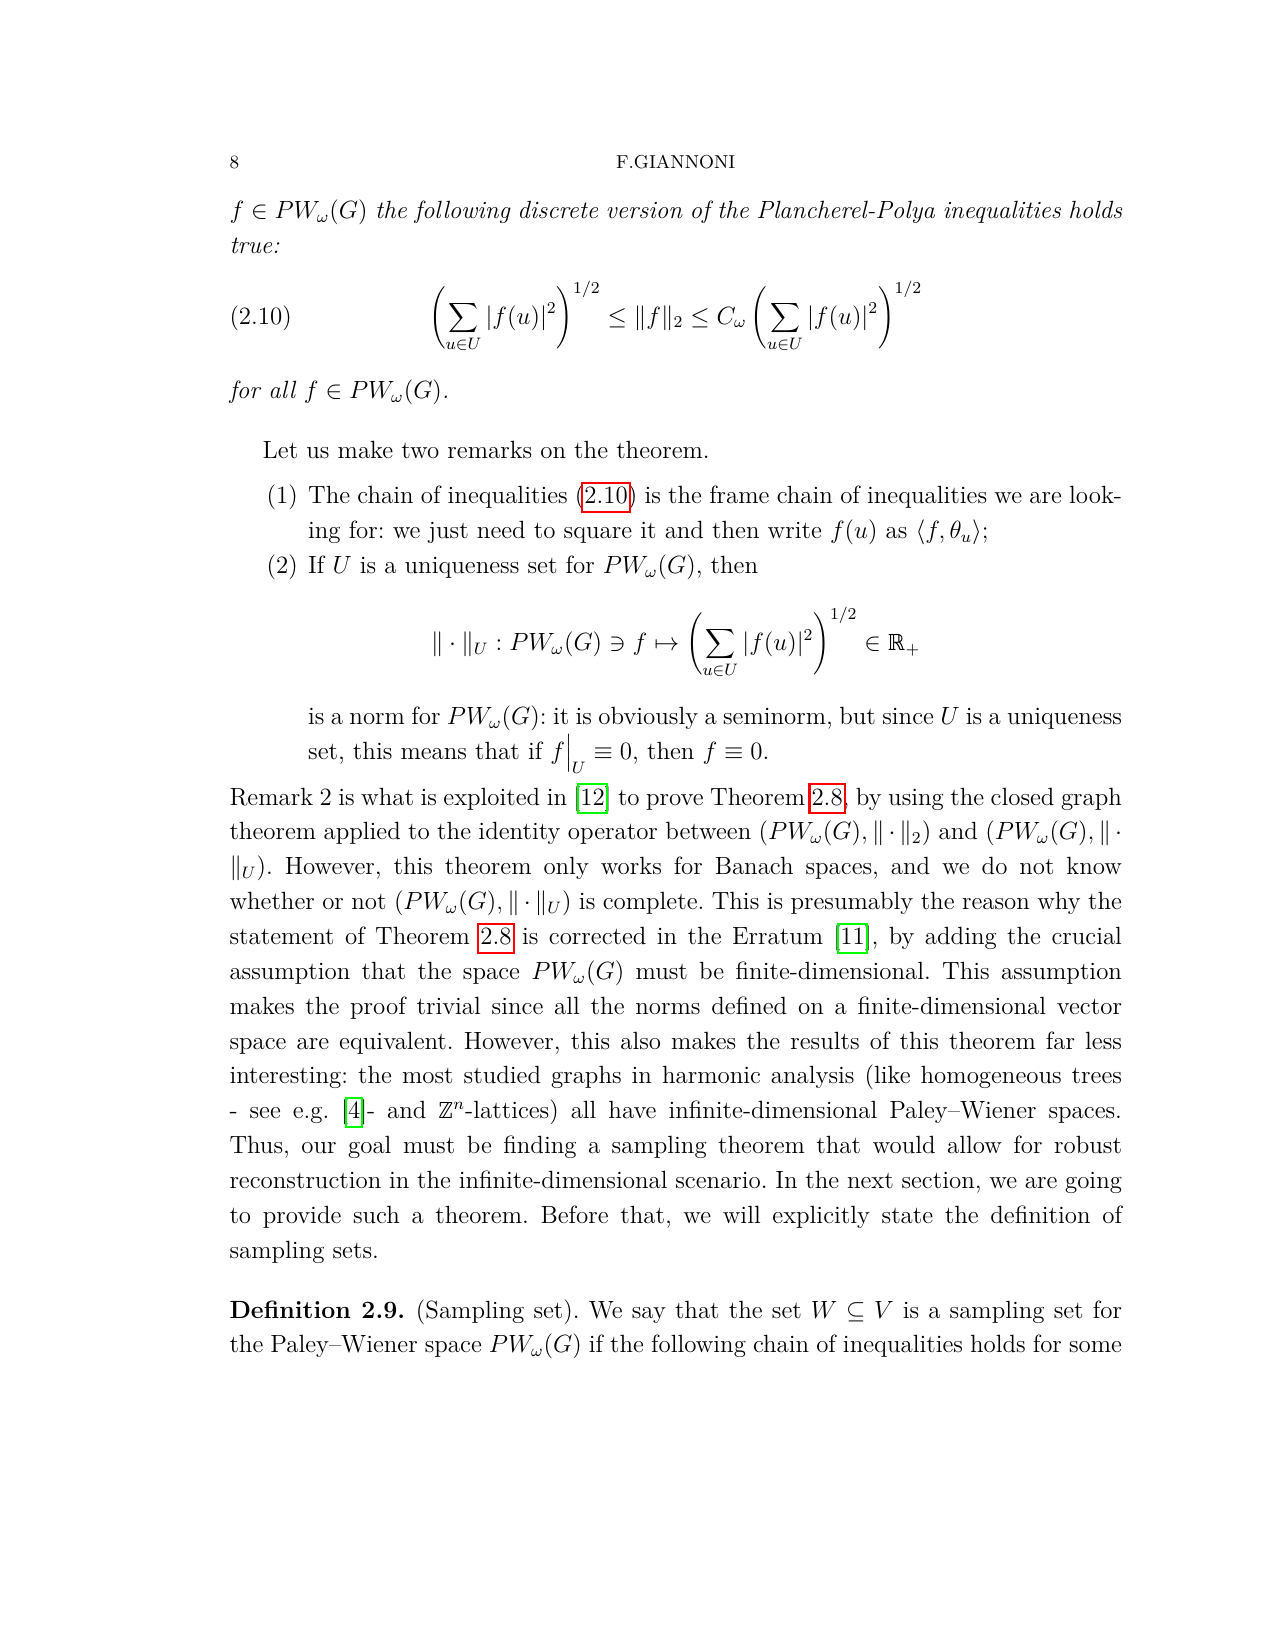
\includegraphics[width=0.91\linewidth,trim=40bp 210bp 40bp 350bp,clip]
 {figures/source_page_8.png}
\end{center}

It then explicitly asks whether uniqueness sets which are not complements of
\(\lambda\)-sets exist (PDF page 10):
\begin{center}
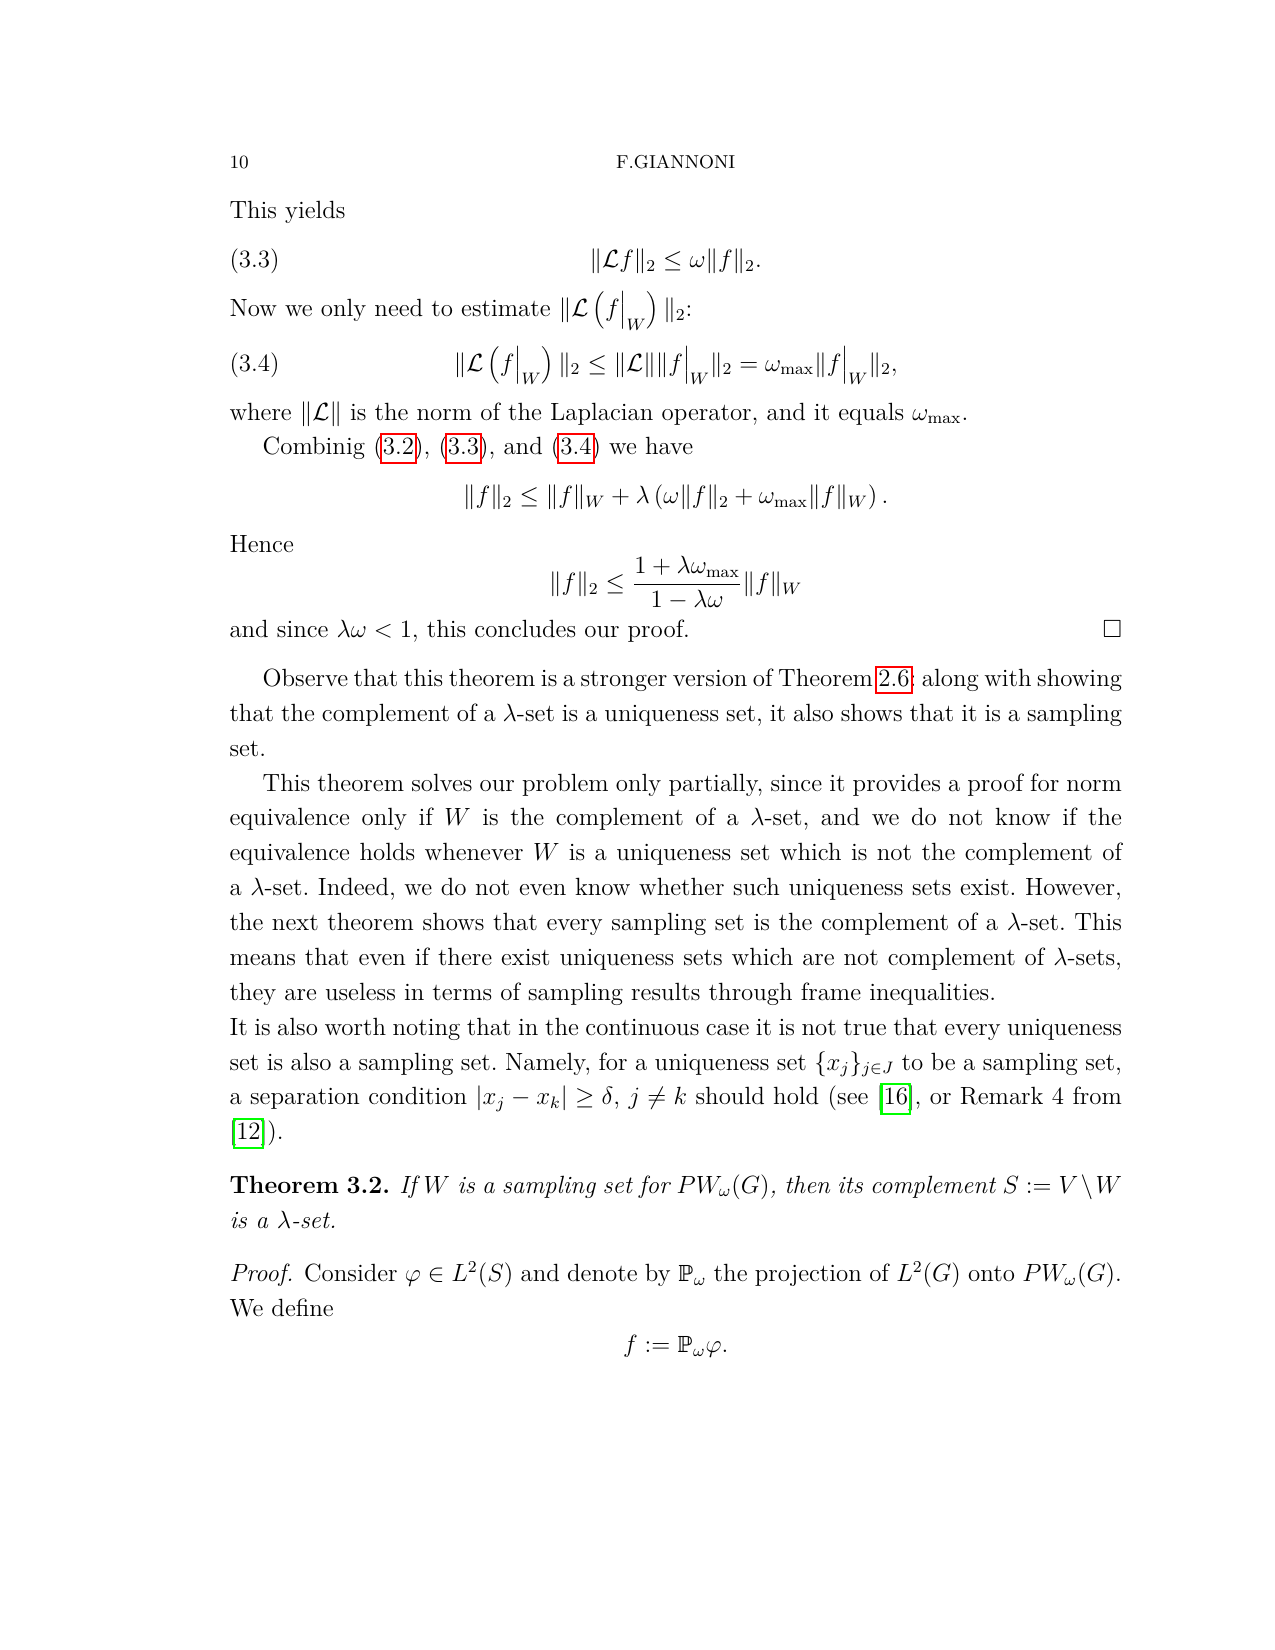
\includegraphics[width=0.91\linewidth,trim=40bp 355bp 40bp 255bp,clip]
 {figures/source_page_10.png}
\end{center}

\begin{thebibliography}{9}
\bibitem{Giannoni}
F.~Giannoni,
\emph{Sampling on Paley--Wiener spaces on graphs, with particular focus on
the infinite-dimensional case}, arXiv:2511.17343v6 (2026), especially
Theorems 2.8, 3.1, 3.2 and the intervening remarks.

\bibitem{MSS}
A.~W.~Marcus, D.~A.~Spielman, and N.~Srivastava,
\emph{Interlacing Families I: Bipartite Ramanujan Graphs of All Degrees},
Ann. of Math. \textbf{182} (2015), 307--325; arXiv:1304.4132.
They prove the existence of infinite families of regular bipartite Ramanujan
graphs of every degree greater than two.
\end{thebibliography}

\end{document}
